\begin{frame}{Model Conditions}
    Multiple regression models 
    \[
        y = \beta_0 + \beta_1x_1 + \beta_2x_2 + \dots + \beta_kx_k + \epsilon
    \]
    depend on the following conditions:
    \begin{enumerate}
        \item Nearly normal residuals.
        \item Constant variability of residuals.
        \item Independence.
        \item Each variable linearly related to the outcome.
    \end{enumerate}
\end{frame}

\begin{frame}{Diagnostic Plots}
    We will consider our final model for the loan data:
    \small{
    \begin{align*}
        \hat{rate} =& 1.921 + 0.974\times\texttt{income\_ver}_{\texttt{source}} + 2.535\times\texttt{income\_ver}_{\texttt{verified}} \\
        &+ 0.021\times\texttt{debt\_income} + 4.896\times\texttt{credit\_util} + 0.387\times\texttt{bankruptcy} \\
        &+ 0.154\times\texttt{term} + 0.228\times\texttt{credit\_check}
    \end{align*}
    }
    and will examine it for any issues with the model conditions.   
\end{frame}

\begin{frame}{Check for Normality}
    As with simple linear regression, there are two ways to check for normality:
    \begin{enumerate}
        \item Histograms
        \item Q-Q Plots
    \end{enumerate}
\end{frame}

\begin{frame}{Check for Normality: Histogram}
    \begin{center}
        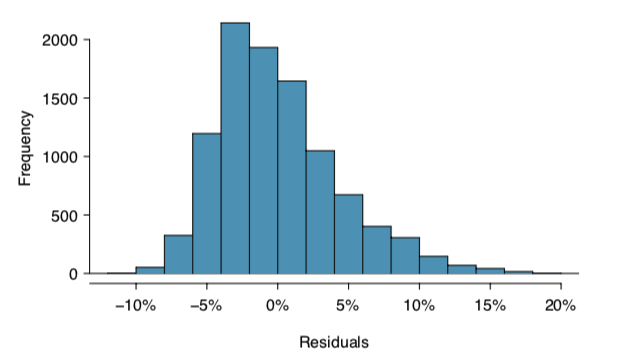
\includegraphics[width=4in]{images/multreghist.png}
    \end{center}
\end{frame}

\begin{frame}{Check for Normality: Q-Q Plots}
    \begin{center}
        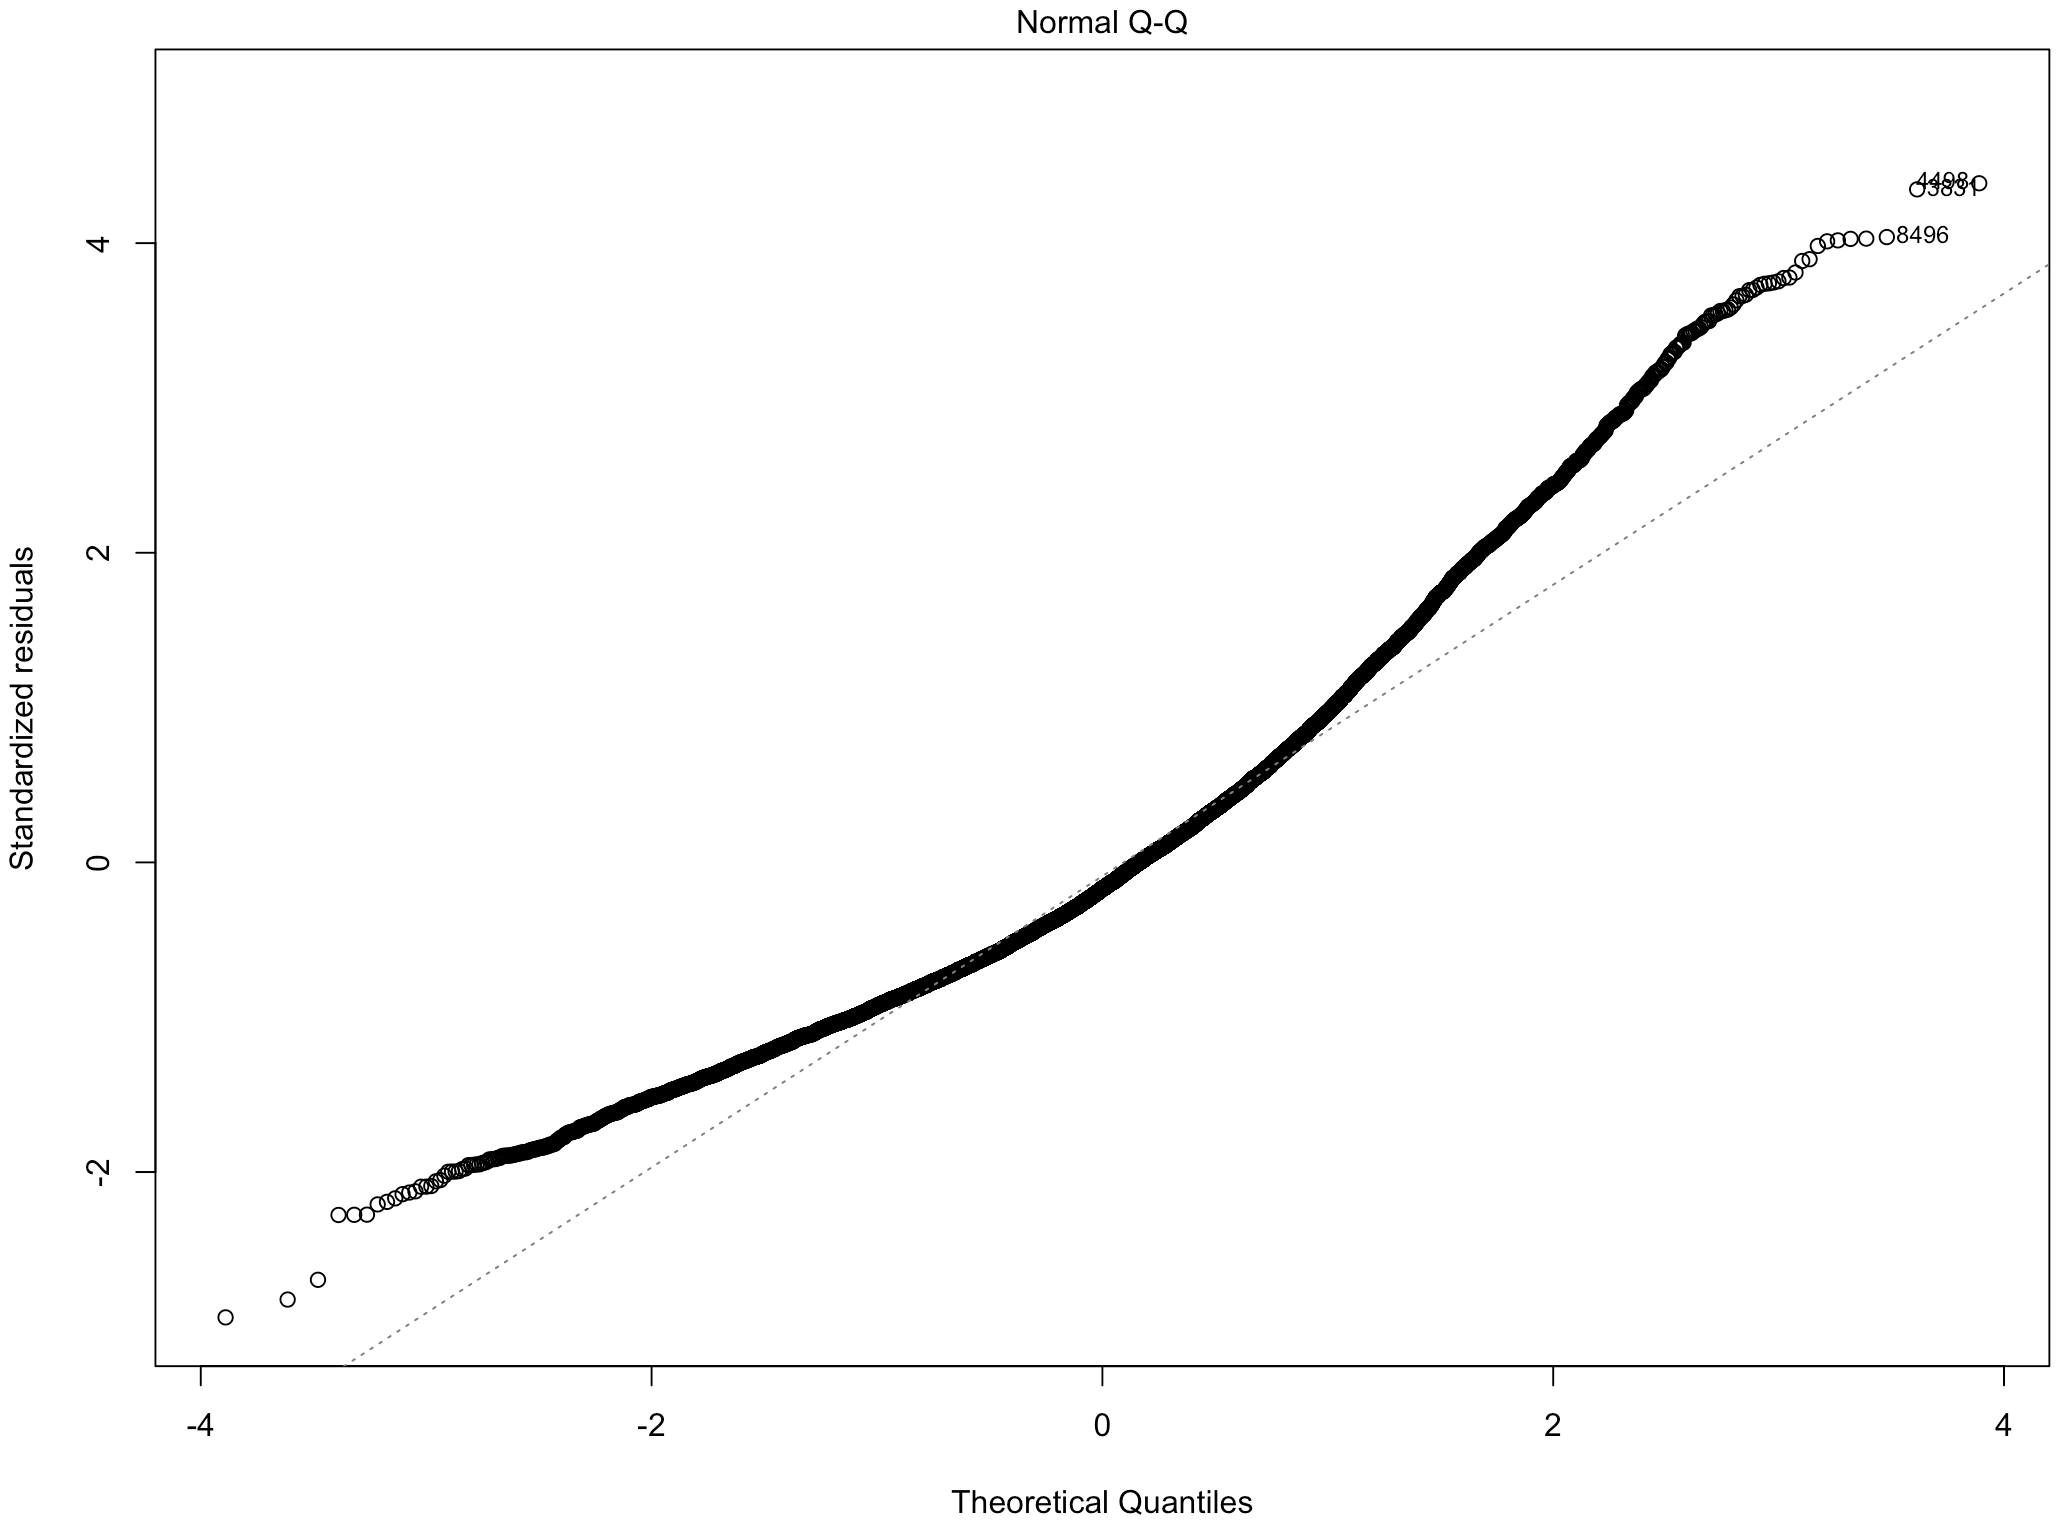
\includegraphics[width=4in]{images/qqmultreg.png}
    \end{center}
\end{frame}

\begin{frame}{The Normality Assumption}
    \begin{itemize}
        \item Since this is such a large dataset (10000 observations), we can relax this assumption some.
        \item \textit{However}, our prediction intervals may not be valid if we do. 
    \end{itemize}
\end{frame}

\begin{frame}{Constant Variance}
    \begin{center}
        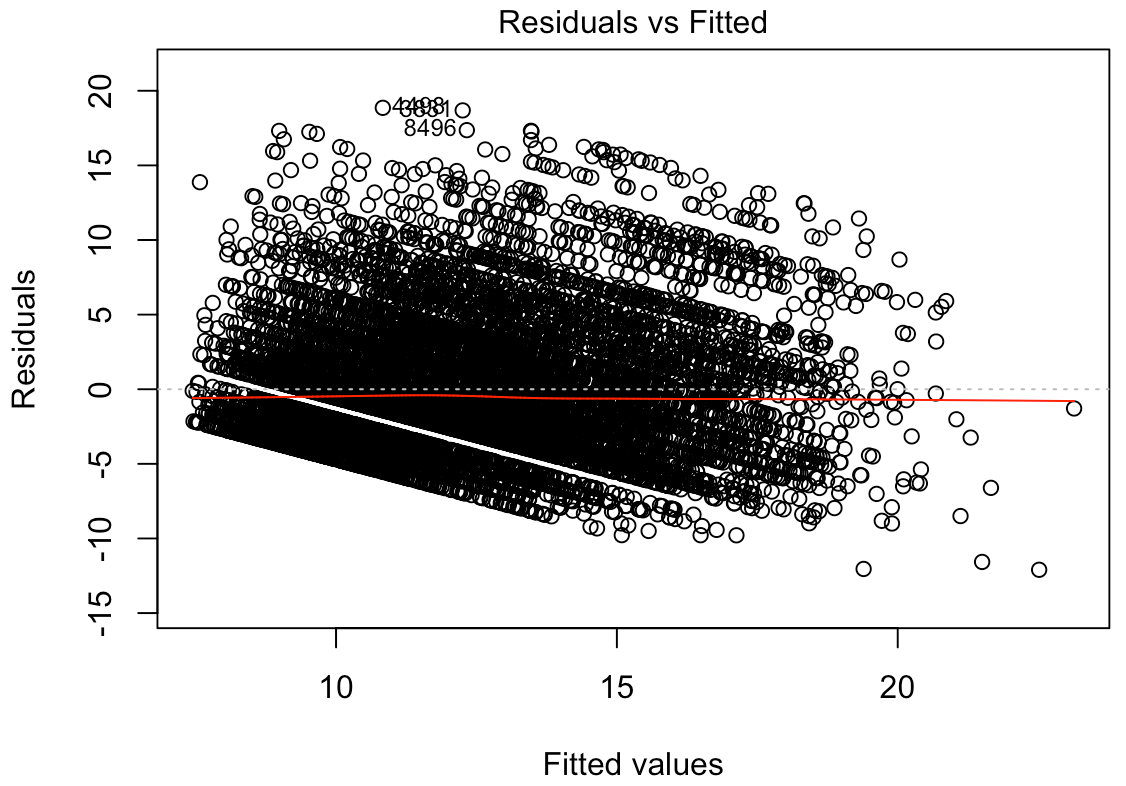
\includegraphics[width=4in]{images/multregconstvar.png}
    \end{center}
\end{frame}

\begin{frame}{Other Useful Diagnostic Plots}
    \begin{itemize}
        \item For data taken in sequence, we might plot \textit{residuals in order of data collection}.
        \begin{itemize}
            \item This can help identify correlation between cases.
            \item If we find connections, we may want to look into methods for \textbf{time series}.
        \end{itemize}
        \item We may also want to look at the residuals plotted against each predictor variable.
        \begin{itemize}
            \item Look for change in variability and patterns in the data.
        \end{itemize}
    \end{itemize}
\end{frame}

\begin{frame}{Residuals Versus Specific Predictor Variables}
    \begin{center}
        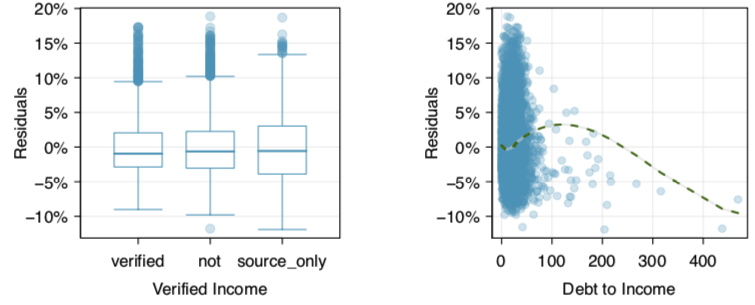
\includegraphics[width=4in]{images/multregvars1.png}
    \end{center}
\end{frame}

\begin{frame}{Residuals Versus Specific Predictor Variables}
    \begin{center}
        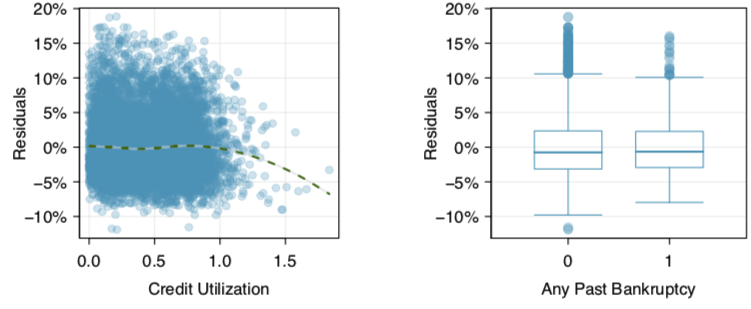
\includegraphics[width=4in]{images/multregvars2.png}
    \end{center}
\end{frame}

\begin{frame}{Residuals Versus Specific Predictor Variables}
    \begin{center}
        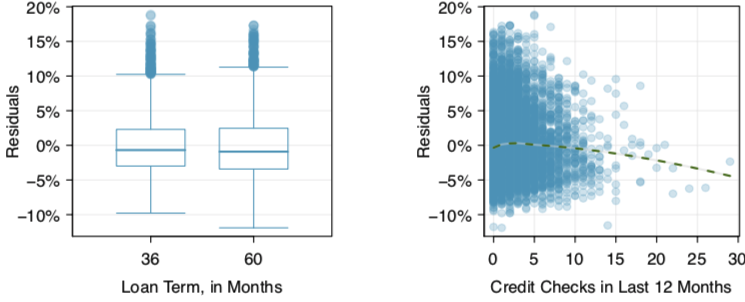
\includegraphics[width=4in]{images/multregvars3.png}
    \end{center}
\end{frame}

\begin{frame}{Now What?}
    \begin{itemize}
        \item If we choose this as our final model, \textit{we must report the observed abnormalities}!
        \item The second option is to look for ways to continue to improve the model.
    \end{itemize}
\end{frame}

\begin{frame}{Transformations}
    One way to improve model fit is to \textit{transform} one or more predictor variables. 
    \begin{itemize}
        \item If a variable has a lot of skew and large values have a lot of leverage, we might try
        \begin{itemize}
            \item Log transformation ($\log{x}$)
            \item Square root transformation ($\sqrt{x}$)
            \item Inverse transformation ($1/x$)
        \end{itemize}
    \end{itemize}
    There are many valid transformations! 
\end{frame}

\begin{frame}{Example: Debt to Income}
    \begin{center}
        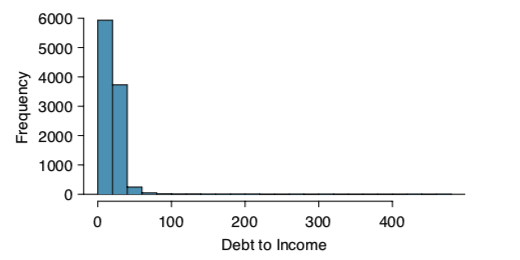
\includegraphics[width=3.5in]{images/debtincomehist.png}
    \end{center}
    \begin{itemize}
        \item We want to deal with this extreme skew.
        \item There are some cases where $\texttt{debt\_to\_income}=0$.
        \item This will make log and inverse transformations infeasible.
    \end{itemize}
\end{frame}

\begin{frame}{Example: Debt to Income}
    First we will try a square root transformation
    \begin{itemize}
        \item We create a new variable, \texttt{sqrt\_debt\_to\_income}
        \[
            \texttt{sqrt\_debt\_to\_income} = \sqrt{\texttt{debt\_to\_income}}
        \]
    \end{itemize}
    We then refit the model with \texttt{sqrt\_debt\_to\_income}.
\end{frame}

\begin{frame}{Example: Debt to Income}
    We will also try a truncation at 50.
    \begin{itemize}
        \item We create a new variable, \texttt{debt\_to\_income\_50}.
        \begin{itemize}
            \item Any values $>50$ are shrunk to 50.
        \end{itemize}
    \end{itemize}
    We then refit the model with \texttt{debt\_to\_income\_50}.
\end{frame}

\begin{frame}{Example: Debt to Income}
    \begin{center}
        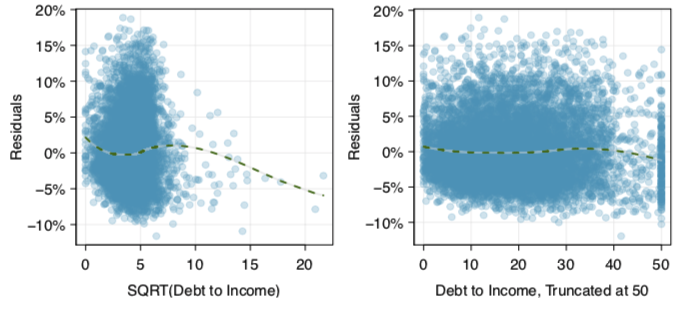
\includegraphics[width=4in]{images/newresids.png}
    \end{center}
    The truncation does a good job fixing the constant variance assumption for this variable.
\end{frame}

\begin{frame}{Example: Debt to Income}
    \begin{itemize}
        \item With the debt to income issue fixed, we should recheck our model assumptions.
        \item We will find the same issues with the other variables.
        \item If we decide that this is our final model, we would need to acknowledge these issues.
    \end{itemize}
\end{frame}

\begin{frame}{Example: Debt to Income}
    The new model is
    \small{
    \begin{align*}
        \hat{rate} =& 1.562 + 1.002\times\texttt{income\_ver}_{\texttt{source}} + 2.436\times\texttt{income\_ver}_{\texttt{verified}} \\
        &+ 0.048\times\texttt{debt\_income} + 4.698\times\texttt{credit\_util} + 0.394\times\texttt{bankruptcy} \\
        &+ 0.153\times\texttt{term} + 0.223\times\texttt{credit\_check}
    \end{align*}
    }
    Notice that the coefficient for \texttt{debt\_income} doubled when we dealt with those high leverage outliers. 
\end{frame}

\begin{frame}{Reporting Results}
    \begin{itemize}
        \item While we may report models that with conditions that are slightly violated,
        \begin{itemize}
            \item ...as long as we acknowledge the violations in our reporting.
        \end{itemize}
        \item we shouldn't report results when conditions are grossly violated.
        \item If familiar methods won't cut it, reach out to an expert.
    \end{itemize}
\end{frame}
